\documentclass[xcolor=x11names,compress]{beamer}

%%%%%%%%%%%%%%%%%%%%%%%%%%%%%%%%%%%%%%%%%%%%%%%%%%%%%%
%%%%%%%%%%%%%%%%%%%%%%%%%%%%%%%%%%%%%%%%%%%%%%%%%%%%%%

\usepackage{graphicx}
\usepackage{tikz}
\usepackage{animate}
\usetikzlibrary{decorations.fractals}
\usepackage{subfigure}

%%%%%%%%%%%%%%%%%%%%%%%%%%%%%%%%%%%%%%%%%%%%%%%%%%%%%%
%%%%%%%%%%%%%%%%%%%%%%%%%%%%%%%%%%%%%%%%%%%%%%%%%%%%%%

\useoutertheme[subsection=false,shadow]{miniframes}
\useinnertheme{default}
\usefonttheme{serif}
\usepackage{palatino}
\usepackage{siunitx}

\setbeamerfont{title like}{shape=\scshape}
\setbeamerfont{frametitle}{shape=\scshape}

\setbeamercolor*{lower separation line head}{bg=DeepSkyBlue4} 
\setbeamercolor*{normal text}{fg=black,bg=white} 
\setbeamercolor*{alerted text}{fg=red} 
\setbeamercolor*{example text}{fg=black} 
\setbeamercolor*{structure}{fg=black} 
 
\setbeamercolor*{palette tertiary}{fg=black,bg=black!10} 
\setbeamercolor*{palette quaternary}{fg=black,bg=black!10} 

\renewcommand{\(}{\begin{columns}}
\renewcommand{\)}{\end{columns}}
\newcommand{\<}[1]{\begin{column}{#1}}
\renewcommand{\>}{\end{column}}
\setbeamertemplate{caption}{\raggedright\insertcaption\par}

%%%%%%%%%%%%%%%%%%%%%%%%%%%%%%%%%%%%%%%%%%%%%%%%%%%%%%
%%%%%%%%%%%%%%%%%%%%%%%%%%%%%%%%%%%%%%%%%%%%%%%%%%%%%%

\usepackage{tikz}
\usetikzlibrary{lindenmayersystems}
\usetikzlibrary[shadings]

\begin{document}
\nocite{*}
\pgfdeclarelindenmayersystem{Sierpinski triangle}{
  \rule{F -> G-F-G}
  \rule{G -> F+G+F}
  }

%%%%%%%%%%%%%%%%%%%%%%%%%%%%%%%%%%%%%%%%%%%%%%%%%%%%%%
%%%%%%%%%%%%%%%%%%%%%%%%%%%%%%%%%%%%%%%%%%%%%%%%%%%%%%

\section{\scshape Introduction}
\begin{frame}
\title{EEG and Chaotic Time Series Analysis}
\author{
	Adam Jump\\
	{\it Salisbury University}\\
}
\date{
	\begin{tikzpicture}[decoration=Koch curve type 2] 
		\draw[DeepSkyBlue4] decorate{ decorate{ decorate{ (0,0) -- (2,0) }}}; 
	\end{tikzpicture}  
	\\
	\vspace{1cm}
	\today
}
\titlepage
\end{frame}

%%%%%%%%%%%%%%%%%%%%%%%%%%%%%%%%%%%%%%%%%%%%%%%%%%%%%%
%%%%%%%%%%%%%%%%%%%%%%%%%%%%%%%%%%%%%%%%%%%%%%%%%%%%%%
\section{\scshape Motivation}
\subsection{frame 1}
\begin{frame}{Why are we interested?}
\begin{itemize}
\item Brain Computer Interfacing
\item Accessibility
\item Applications in Artificial Intelligence
\item Prediction of Chaotic Time Series
\end{itemize}
\begin{figure}
\centering
\subfigure[\text{Channel 1 Spectrogram}]{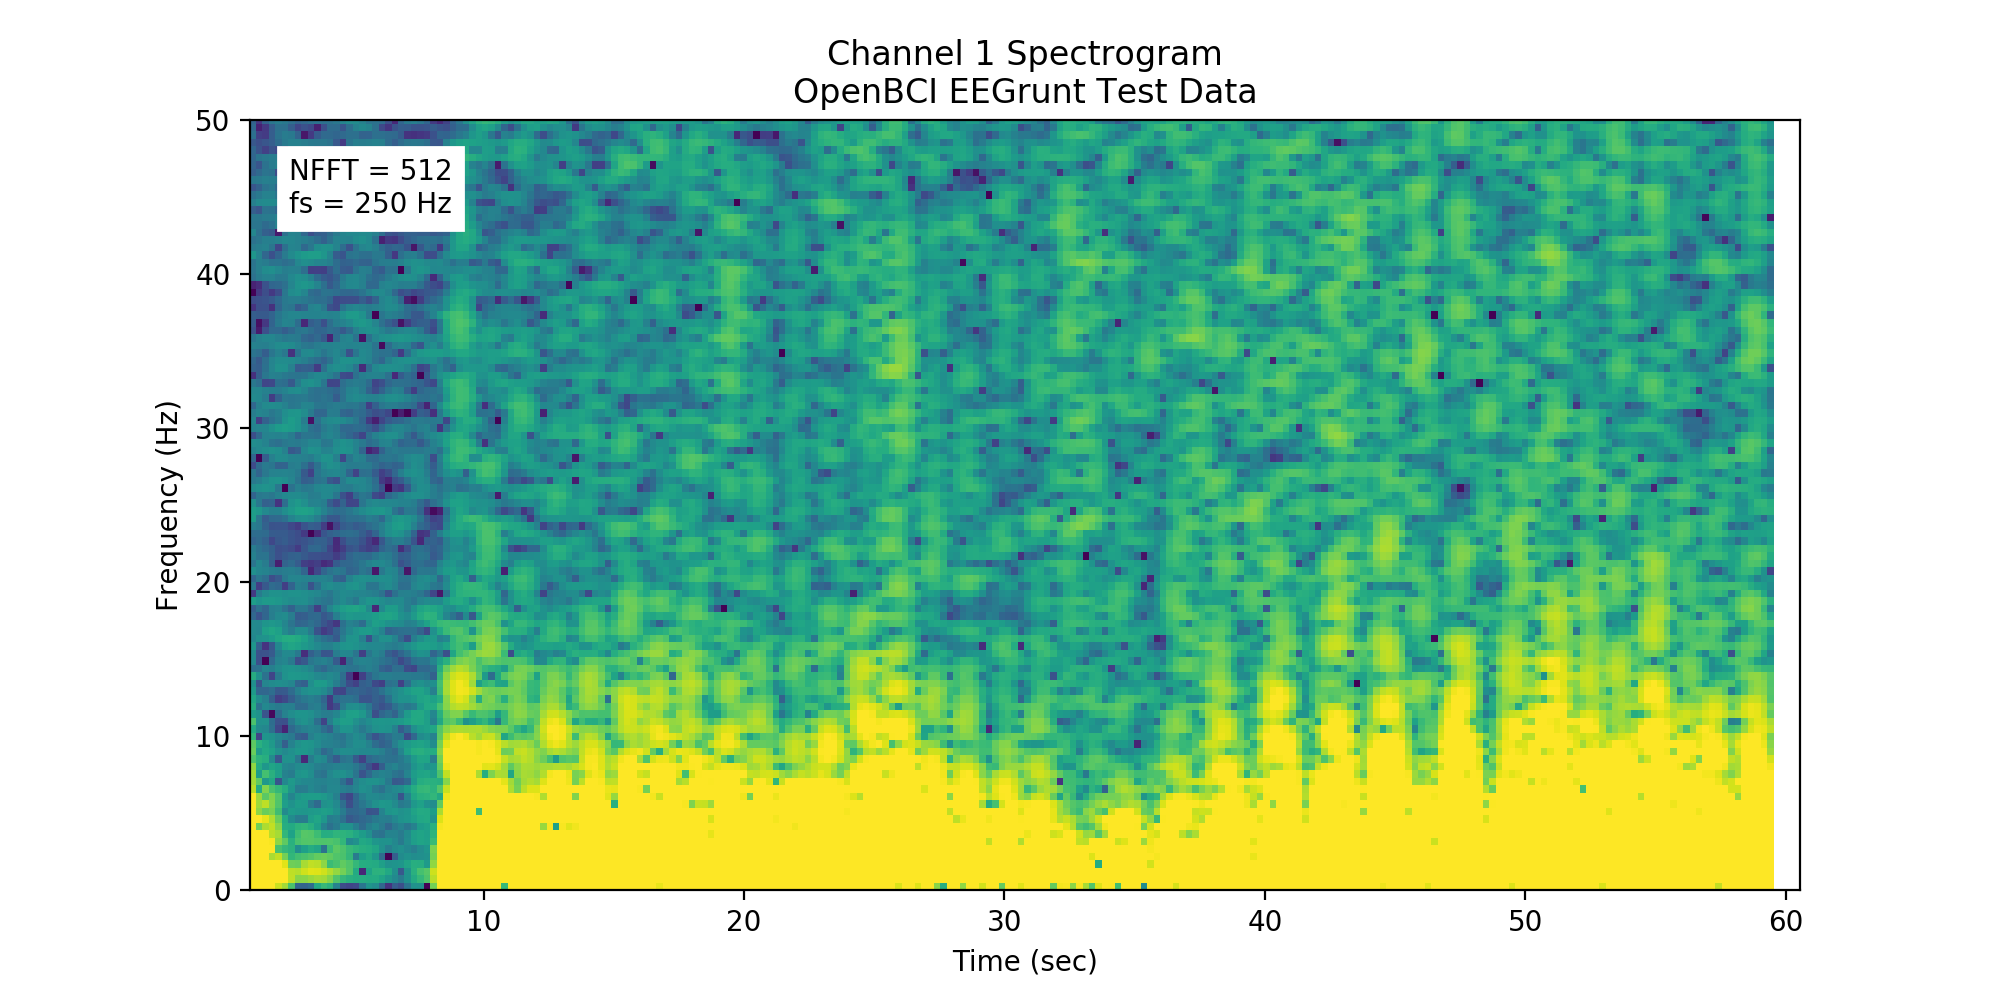
\includegraphics[width=1.6in]{Channel_1_Spec_Blink_Test.png}}
\hspace{10mm}
\subfigure[\text{Channel 2 Spectrogram}]{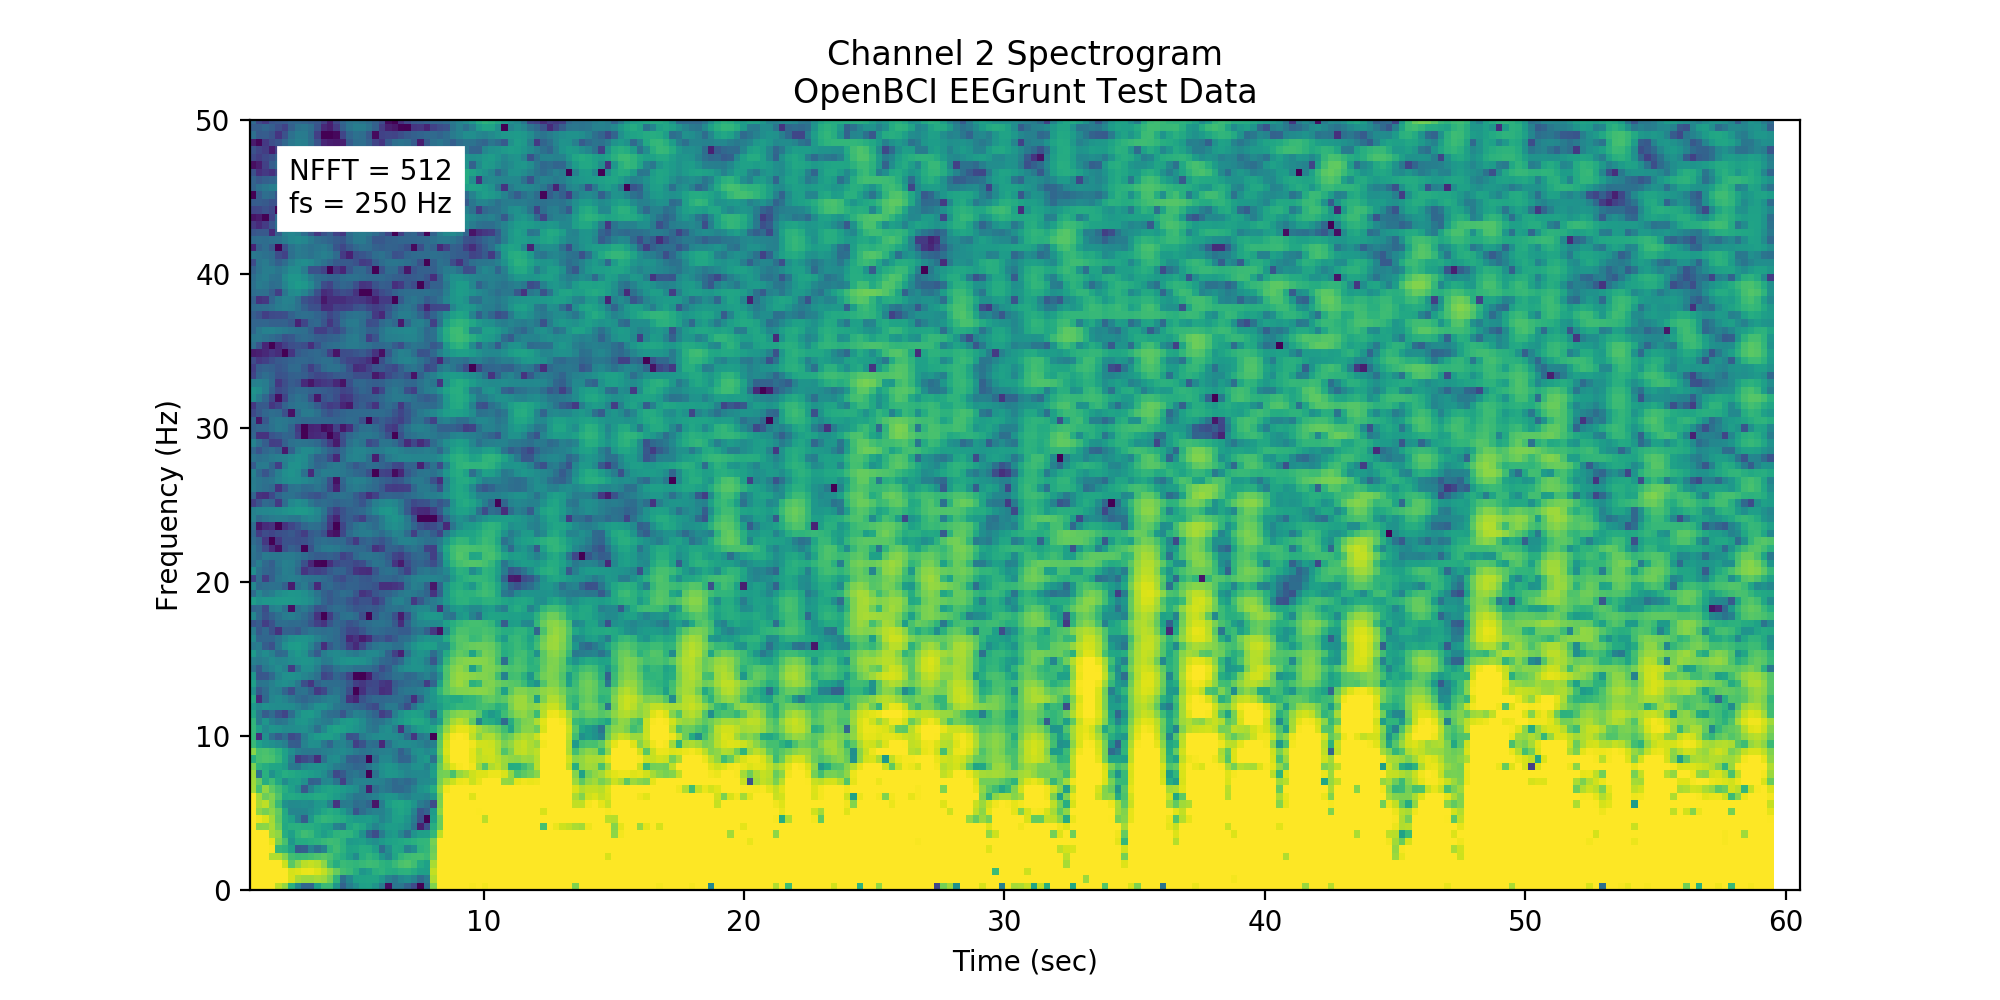
\includegraphics[width=1.6in]{Channel_2_Spec_Blink_Test.png}}
\hspace{10mm}
\end{figure}
\end{frame}

%%%%%%%%%%%%%%%%%%%%%%%%%%%%%%%%%%%%%%%%%%%%%%%%%%%%%%
%%%%%%%%%%%%%%%%%%%%%%%%%%%%%%%%%%%%%%%%%%%%%%%%%%%%%%
\section{\scshape Analysis}
\subsection{frame 2}
\begin{frame}{Translation from the Time Domain}

\begin{itemize}
\item
8 electrodes giving us row vectors, $$f(t) = (x_1,x_2,x_3,x_4,x_5,x_6,x_7,x_8),$$ $$x_i=x(t+i\tau)$$
\item
Utilizing the \textit{Discrete Fourier Transform}, $$F_n=\sum_{k=0}^{N-1}X_k  \cdot  e^{-2\pi i n k/N}$$
\item
Multiplying by low and high pass filters, $$\frac{t}{\tau + t},\frac{\tau}{t+\tau}$$
\end{itemize}
\end{frame}

%%%%%%%%%%%%%%%%%%%%%%%%%%%%%%%%%%%%%%%%%%%%%%%%%%%%%%
%%%%%%%%%%%%%%%%%%%%%%%%%%%%%%%%%%%%%%%%%%%%%%%%%%%%%%

\subsection{frame 3}
\begin{frame}{Frequency Domain}
\begin{itemize}
\item Why look at frequency?
\end{itemize}
\begin{figure}[h]
   \centering
   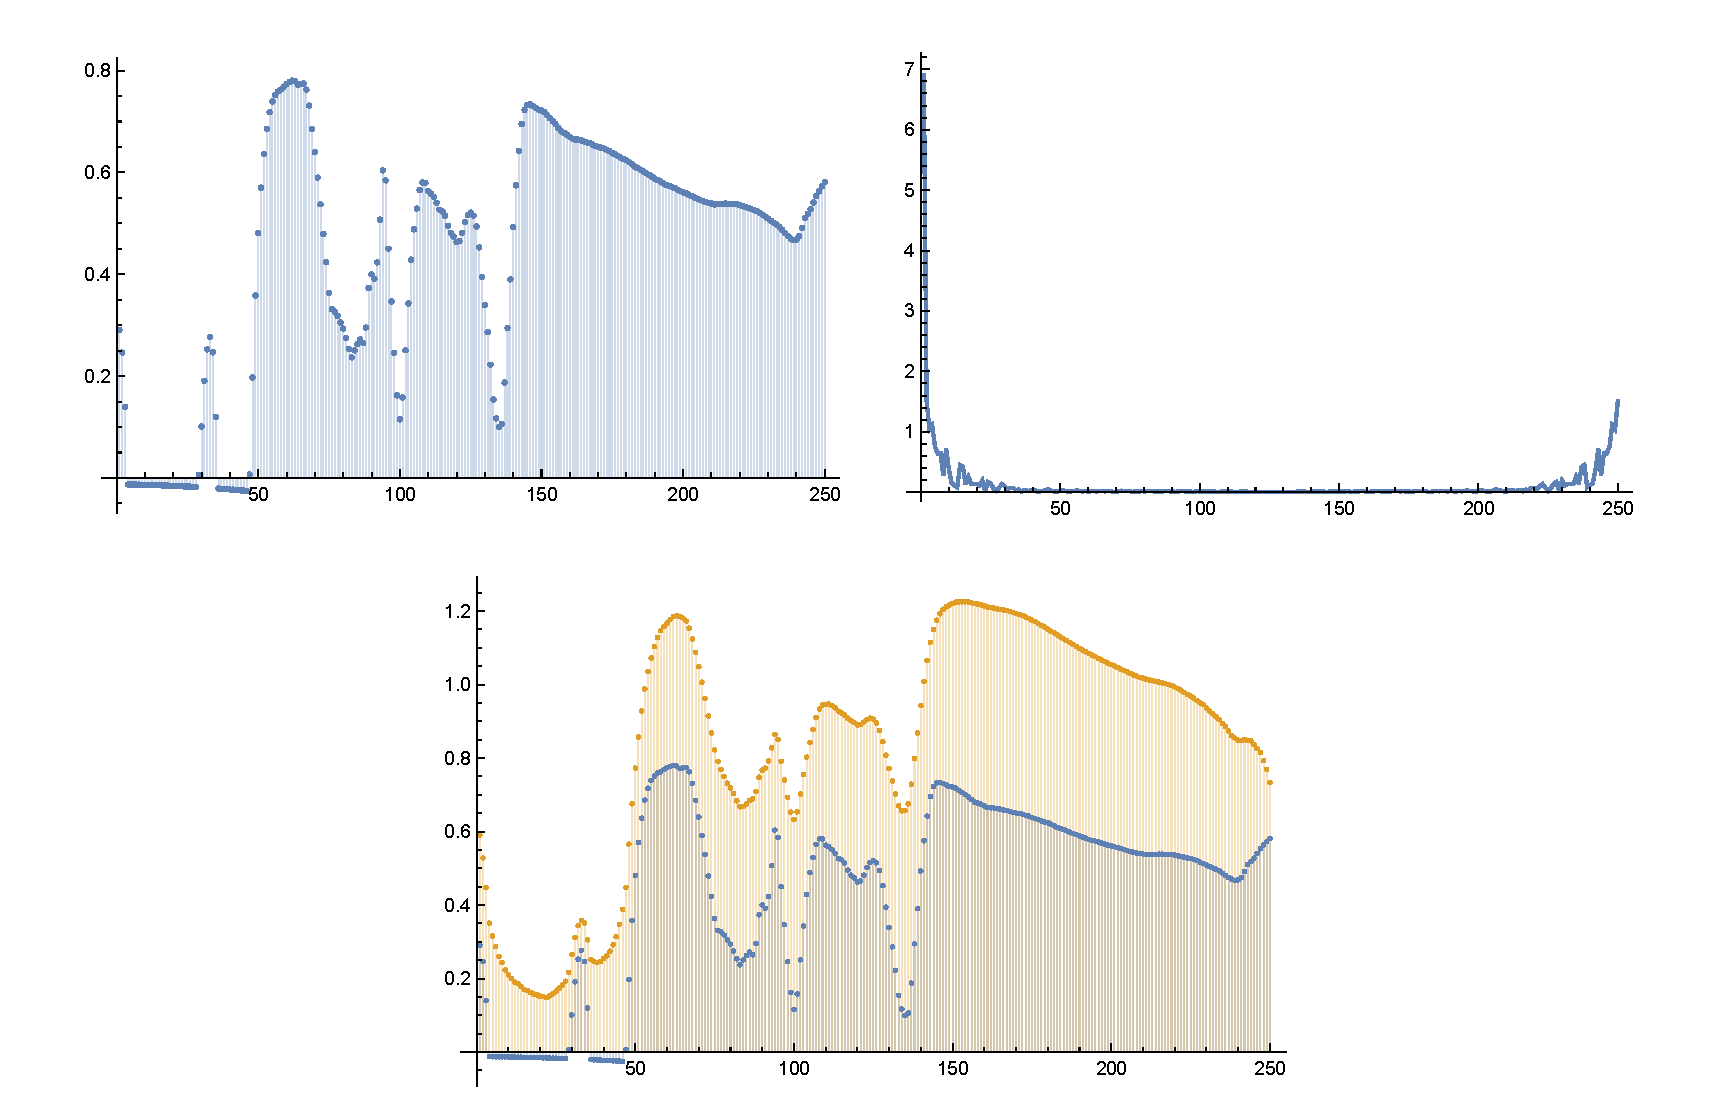
\includegraphics[width=3in]{Fourier.pdf} 
   \label{fig:example}
\end{figure}
\end{frame}

%%%%%%%%%%%%%%%%%%%%%%%%%%%%%%%%%%%%%%%%%%%%%%%%%%%%%%
%%%%%%%%%%%%%%%%%%%%%%%%%%%%%%%%%%%%%%%%%%%%%%%%%%%%%%

\subsection{frame 4}
\begin{frame}{Time-Frequency Domain (wavelets)}
\begin{itemize}
\item The individual wavelet defined as, $$\psi^{a,b}(x)=\left\vert a\right\vert^{-1/2}\psi \left(\frac{x-b}{a}\right)$$
\item which gives, $$W_{\psi}(f)(a,b)=\frac{1}{\sqrt{a}}\int_{-\infty}^{\infty}f(t)\psi \left(\frac{t-b}{a}\right)d\,t$$
\end{itemize}
\begin{center}
\animategraphics[loop,controls,width=2in]{12}{Data-}{1}{236}
\end{center}
\end{frame}

%%%%%%%%%%%%%%%%%%%%%%%%%%%%%%%%%%%%%%%%%%%%%%%%%%%%%%%
%%%%%%%%%%%%%%%%%%%%%%%%%%%%%%%%%%%%%%%%%%%%%%%%%%%%%%%

\subsection{frame 5}
\begin{frame}{Artifact Removal and return to Linearity}
\begin{itemize}
\item For all $f(t)$ we want to find $\mathbf{M}$ such that $f(t)\mathbf{M}=\mathbf{s}$ where all $\mathbf{s}$ are maximally independent
\item Generally referred to as an \textit{independent component analysis} and used in unsupervised machine learning
\end{itemize}
\begin{figure}[h] 
   \centering
   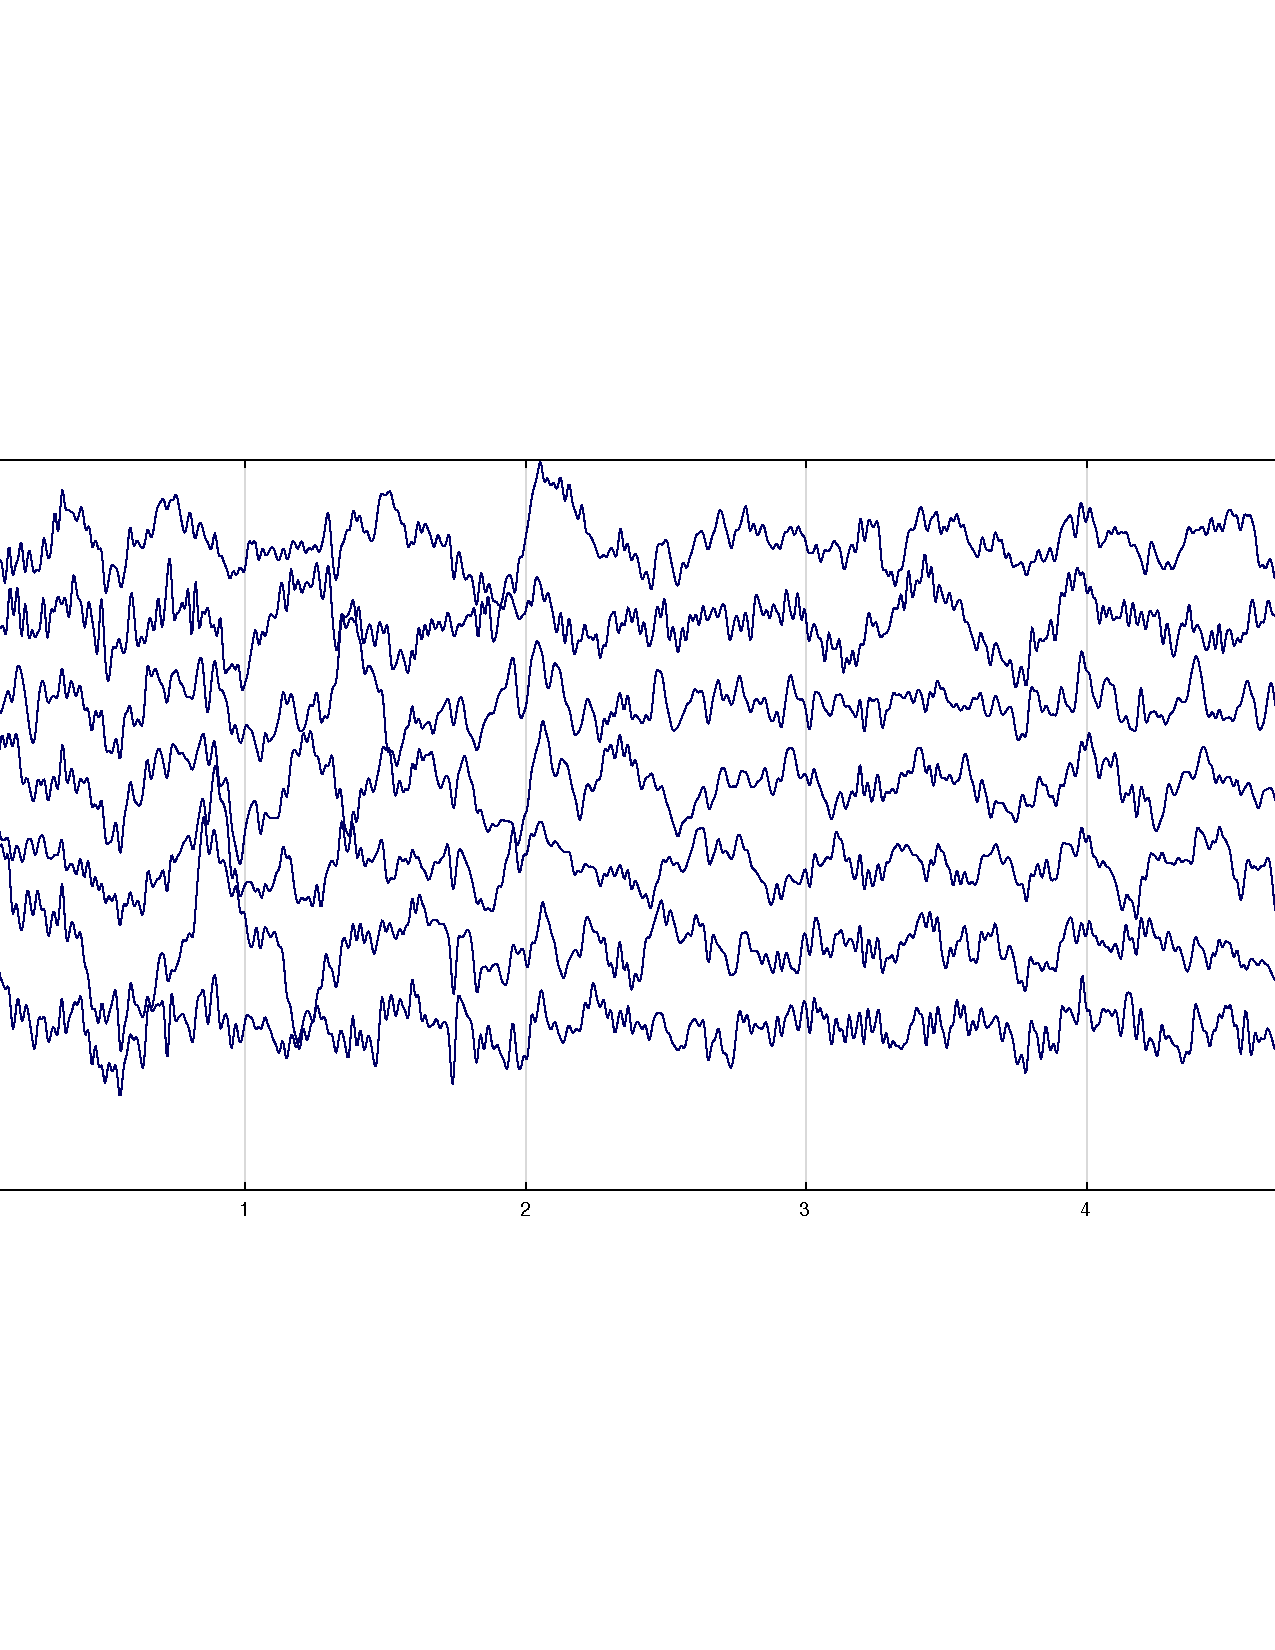
\includegraphics[width=2in]{Time_Series.pdf} 
   \caption{Processed Time-Series Data}
   \label{fig:example}
\end{figure}
\end{frame}

%%%%%%%%%%%%%%%%%%%%%%%%%%%%%%%%%%%%%%%%%%%%%%%%%%%%%%%
%%%%%%%%%%%%%%%%%%%%%%%%%%%%%%%%%%%%%%%%%%%%%%%%%%%%%%%

\subsection{frame 6}
\begin{frame}{Chaotic Time-Series Prediction}
\begin{itemize}
\item Nonlinear autoregressive exogenus model (NARX)
\item Algebraically stated as $y(t)  = N[y_{t-1}, y_{t-2}, y_{t-3},\dots,u_{t},u_{t-1}, \dots] +\epsilon_{t}$
\end{itemize}
\begin{figure}[h]
   \centering
   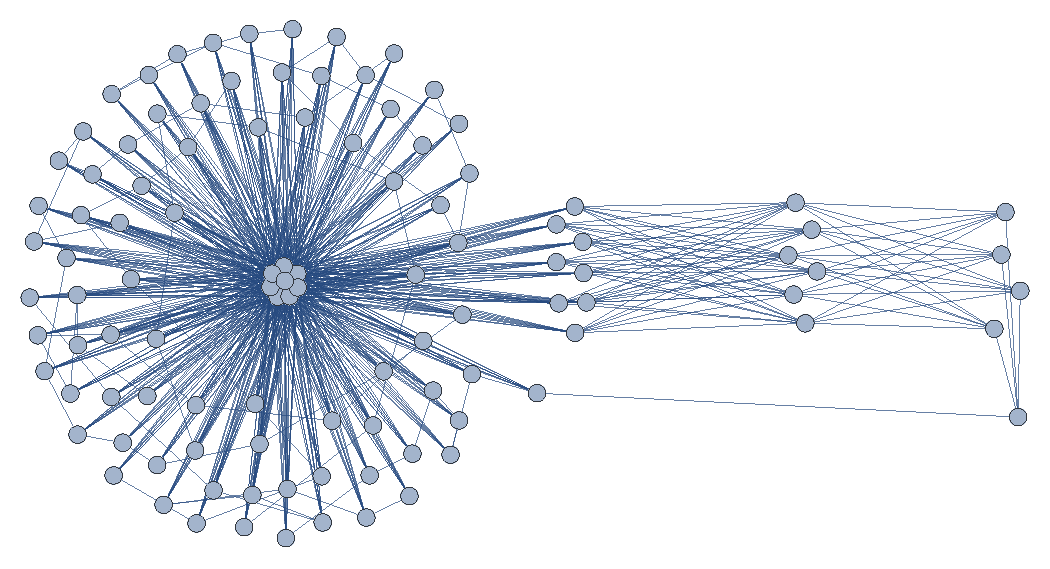
\includegraphics[width=2in]{narx.pdf}
   \label{fig:example}
\end{figure}
\end{frame}

%%%%%%%%%%%%%%%%%%%%%%%%%%%%%%%%%%%%%%%%%%%%%%%%%%%%%%%
%%%%%%%%%%%%%%%%%%%%%%%%%%%%%%%%%%%%%%%%%%%%%%%%%%%%%%%

%\subsection{frame 7}
%\begin{frame}{Proposal}
%\textbf{Proposed Immediate Team Goals}
%	\begin{itemize}
%	\item Game Design Team
%		\begin{itemize}
%		\item That's all you, Nathan
%		\end{itemize}
%	\item Brain/Computer Interface Team
%		\begin{itemize}
%		\item Streaming into Unity/Feature detection/Signal Processing~\cite{noauthor_frequency_nodate}
%		\end{itemize}
%	\item Artificial Intelligence Team
%		\begin{itemize}
%		\item Solved Turing Machine problems for comparison with human solutions
%		\end{itemize}
%	\item Core Integration Team
%		\begin{itemize}
%		\item Design a grid that receives two flags to move one tile of the grid left or right
%		\end{itemize}
%	\item Artwork Team
%		\begin{itemize}
%		\item Tileset for use in Unity
%		\end{itemize}
%	\item Music and Sound Team
%		\begin{itemize}
%		\item That's all you, Thomas
%		\end{itemize}
%	\end{itemize}
%\end{frame}

%%%%%%%%%%%%%%%%%%%%%%%%%%%%%%%%%%%%%%%%%%%%%%%%%%%%%%%
%%%%%%%%%%%%%%%%%%%%%%%%%%%%%%%%%%%%%%%%%%%%%%%%%%%%%%%

%\subsection{frame 8}
%\begin{frame}{Proposal}
%\textbf{Proposed Future Team Goals}
%	\begin{itemize}
%	\item Game Design Team
%		\begin{itemize}
%		\item Proactive Recreation/Make these tests feel like a game
%		\end{itemize}
%	\item Brain/Computer Interface Team
%		\begin{itemize}
%		\item Build different headset sizes/ improve comfort/ IRB approval
%		\end{itemize}
%	\item Artificial Intelligence Team
%		\begin{itemize}
%		\item From different Turing Machine solutions, create a system that writes its own algorithms
%		\end{itemize}
%	\item Core Integration Team
%		\begin{itemize}
%		\item Minimize interaction with OpecBCI\_GUI/ Optimize data handling/ Integrating the team goals
%		\end{itemize}
%	\item Artwork Team
%		\begin{itemize}
%		\item Design voxel set
%		\end{itemize}
%	\item Music and Sound Team
%		\begin{itemize}
%		\item Indications of correct problem solving/ incorrect problem solving (a continuous problem)
%		\end{itemize}
%	\end{itemize}
%\end{frame}
%
%%%%%%%%%%%%%%%%%%%%%%%%%%%%%%%%%%%%%%%%%%%%%%%%%%%%%%%%
%%%%%%%%%%%%%%%%%%%%%%%%%%%%%%%%%%%%%%%%%%%%%%%%%%%%%%%%
%
%\subsection{frame 9}
%\begin{frame}{Comments}
%Thoughts?
%	\begin{figure}[h]
%		\centering
%		\subfigure[Data]{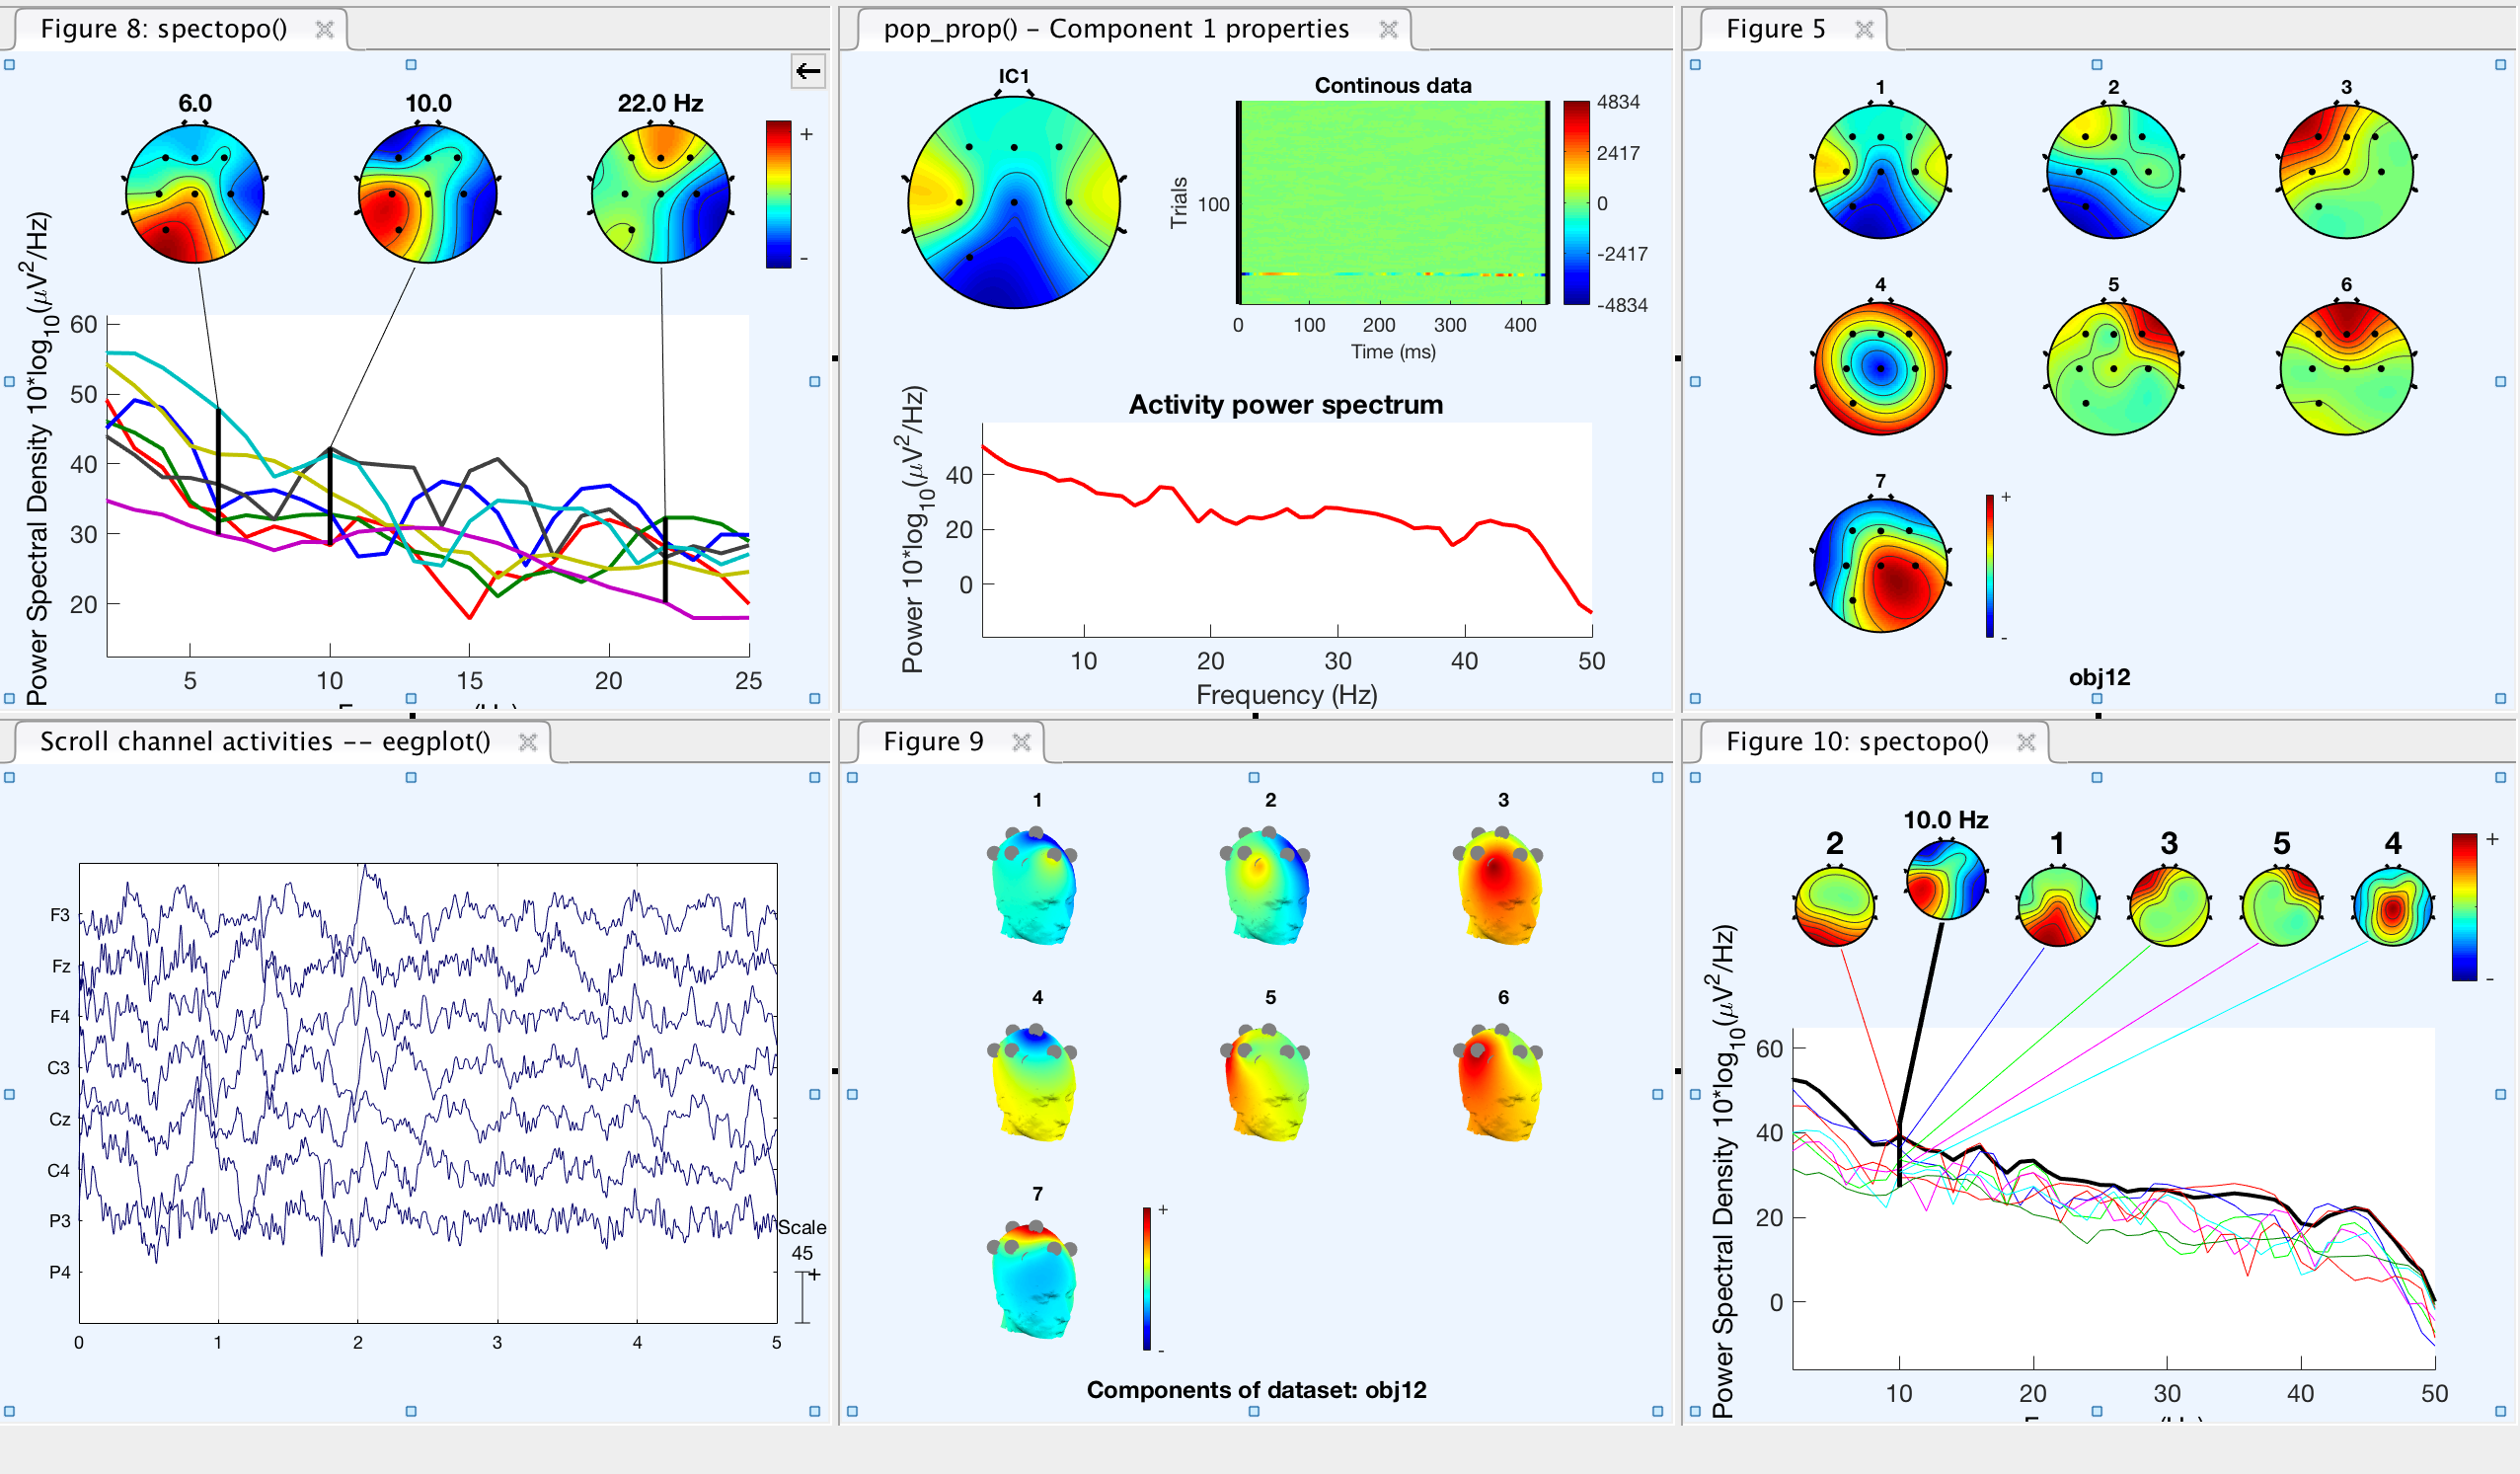
\includegraphics[width=3in]{Untitled.png}}
%		\hspace{10mm}
%	\end{figure}
%\end{frame}

%%%%%%%%%%%%%%%%%%%%%%%%%%%%%%%%%%%%%%%%%%%%%%%%%%%%%%%
%%%%%%%%%%%%%%%%%%%%%%%%%%%%%%%%%%%%%%%%%%%%%%%%%%%%%%%

\section{\scshape References}
\subsection{last}
\begin{frame}[shrink=50]{References}
	\bibliographystyle{alpha}
	\bibliography{Citations.bib}
\end{frame}

%%%%%%%%%%%%%%%%%%%%%%%%%%%%%%%%%%%%%%%%%%%%%%%%%%%%%%%
%%%%%%%%%%%%%%%%%%%%%%%%%%%%%%%%%%%%%%%%%%%%%%%%%%%%%%%

\end{document}